\documentclass{article}
\usepackage[margin=1in]{geometry}
\usepackage{setspace}
\usepackage{amsmath}
\usepackage{amssymb}
\usepackage{physics}
\usepackage{graphicx}
\usepackage{relsize}

\title{CS 180 Midterm}
\author{Jiaping Zeng}
\date{11/2/2020}

\begin{document}
\setstretch{1.5}

\newpage
\maketitle

\newpage
\begin{itemize}
    \item [P1]
          \textbf{Algorithm}: Assume that there is a path between the starting node and the target node.
          \begin{itemize}
              \item [1.] Start at arbitrary node, traverse through its adjacent nodes.
              \item [2.] Repeat the previous step for all the adjacent nodes until the target is found.
          \end{itemize}
          \textbf{Proof of correctness}: By contradiction. Suppose that the algorithm does not find the target node. Then it means that the algorithm missed the target node during its traversal away from the starting node. However, since our algorithm exhausts every possible path within the graph, this must mean that the graph is disconnected and there is no path between the starting node and the target node, which contradicts our initial assumption that there is a path between them. Therefore this algorithm is correct.\\
          \textbf{Time complexity}: $O(m)$ for $m$ edges since we are traversing through all edges.
\end{itemize}

\newpage
\begin{itemize}
    \item [P2]
          \textbf{Algorithm}:
          \begin{itemize}
              \item [1.] Sort list of tasks and store the start and end times. In addition let $max$ be the max number of tasks at a time.
              \item [2.] Traverse through the sorted list, increment task count for each task started and decrement task count for each task ended. Update $max$ when task count exceeds it.
              \item [3.] Return $max$ as the min number of processors needed.
          \end{itemize}
          \textbf{Proof of correctness}: By contradiction; suppose the algorithm returns a number that is not the minimum number of processors needed. Then it must have overcounted the number of tasks at at least one moment in time. However by sorting  and decrementing on task end we cannot have overcounted.\\
          Now suppose the algorithm returns a number that is not enough. Since all tasks started are included in our list and we have incremented task count each time one starts, while decrementing only when the task ends, we could not have undercounted. Therefore this algorithm is correct by contradiction.
          \textbf{Time complexity}: $O(n\log n)$ since we have to sort the list which is at least $O(n\log n)$.
\end{itemize}

\newpage
\begin{itemize}
    \item [P3]
          \textbf{Algorithm}:
          \begin{itemize}
              \item [1.] Let $a,b$ be two colors; we start by coloring an arbitrary node $a$, and mark the node as visited.
              \item [2.] Traverse to the adjacent nodes and color them $b$, skip if the node is marked as visited.
              \item [3.] Repeat the previous step for each of the nodes visited while alternating the color for each level.
              \item [4.] If in the end we have adjacent nodes with the same color, return false; else return true.
          \end{itemize}
          \textbf{Proof of correctness}: By contradiction; suppose the algorithm returns true when the graph is not 2-colorable. But since the algorithm colored the graph along the way without having adjacent nodes with the same color, the result graph would satisfy the definition of 2-colorable.\\
          Now suppose the algorithm returns false when the graph is 2-colorable. Then there exists a way to color the graph in a way that no adjacent nodes have the same color. But since our algorithm has traversed to each node and alternatingly colored each layer, it would have found such coloring pattern.\\
          Therefore this algorithm is correct by contradiction.\\
          \textbf{Time complexity}: $O(n+m)$ for $n$ nodes and $m$ edges since we visit each node and each edge exactly once.
\end{itemize}

\newpage
\begin{itemize}
    \item [P4] As follows:
    \begin{center}
        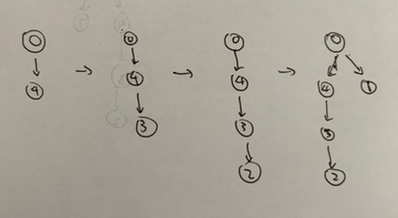
\includegraphics[width=6in]{p4.png}
    \end{center}
\end{itemize}

\newpage
\begin{itemize}
    \item [P5]
          \textbf{Algorithm}:
          \begin{itemize}
              \item [1.] Divide the list in half.
              \item [2.] If each sublist has length $\leq 2$, perform the following:
                    \begin{itemize}
                        \item [-] Compare the two elements and store the max and min.
                        \item [-] In case of length 1 sublist, store the only element as both max and min.
                    \end{itemize}
              \item [3.] Else if each sublist has length $>2$, repeat steps 1-3 for each sublist and compare the max and min found there.
              \item [4.] Return the max and min found from the previous step.
          \end{itemize}
          \textbf{Proof of correctness}: By induction. We will show that the algorithm works for a list of length 2 as the base case, and by the inductive step that it will work for longer lists as well.\\
          Base case: $n=2$, the algorithm divides the list into two elements which are the only element of its sublist. So by step 2.2 they are stored as both the max and the min of their respective sublist. Then they are compared and returned which indeed gives us the correct values.\\
          Inductive step: Suppose that the algorithm works for a list of length $n$, we will show that it also works for a list of length $n+1$. We can examine the following two cases:
          \begin{itemize}
              \item [-] $n$ is odd: after we recursively divide the list of length $n$ down to sublists with length $\leq 2$, we will have exactly one sublist with length 1. So for a list of $n+1$ elements we can simply place the new element into the sublist with length 1, then by the inductive hypothesis we will have the correct result.
              \item [-] $n$ is even: after we recursively divide the list, we will have sublists of length $=2$. So the new element is placed in its own sublist which then gets returned as both the max and min and compared with the rest. Then by inductive hypothesis we will also have the correct result here.
          \end{itemize}
          Therefore this algorithm is correct by induction.\\
          \textbf{Number of comparisons}: We have at most $2(n/2-1)$ comparisons for sublists of length $\leq 2$. Then comparing the parent lists gives us $2(n/4-1)$ comparisons. Therefore we have $2n(2^{-1}+2^{-2}+2^{-3}+\ldots)-\frac{1}{2}n$ comparisons which by infinite series gives us $\frac{3n}{2}$ comparisons.
\end{itemize}
\end{document}